\newpage

\section{Analýza problematiky}
\lipsum[3]

\subsection{Podsekcia 1}
\lipsum 

Segmentácia obrazu sa v dnešnej dobe využíva veľmi často v medicíne napr. pri snímkach mozgu \cite{5}, pri detekcií objektov, pri rozpoznávaní tváre \cite{6} a v neposlednom rade pri vyhľadávaní snímok na základe obsahu \cite{7}.

\subsubsection{Podsekcia 2}
Zoznam:
\begin{my_itemize}
	\item Položka 1
	\item Položka 2
\end{my_itemize}

\paragraph{Podsekcia 3}
\lipsum[1]

\begin{figure}[H]
	\begin{center}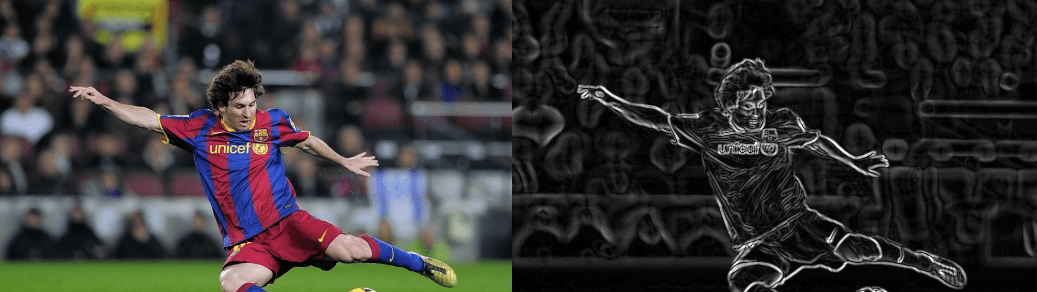
\includegraphics[scale=0.35]{figure3}\end{center}
	\caption[Sobel operátor]{Ukážka pred a po aplikácií Sobel operátora pri detekcií hrán\footnotemark 
		 
	}\label{f3}
\end{figure}
\footnotetext{Zdroj: WeekMedia, \href{http://opencvpython.blogspot.sk/2012/06/image-derivatives-sobel-and-scharr.html}{Abid Rahman K}}

\lipsum[1]

\paragraph{Podsekcia 3} \label{podobnost}

S algoritmom prichádza funkcia energie $E(s)$, ktorá ohodnocuje kvalitu špecifického rozdelenia obrazu a má tvar:
\begin{equation} \label{ener}
	E(s) = H(s) + \gamma G(s)
\end{equation}
